\documentclass{article}% use option titlepage to get the title on a page of its own.
\usepackage{float}
\usepackage{graphicx}
\graphicspath{ {./images/} }
\usepackage{blindtext}
\title{\vspace{-3.0cm} \textbf{\LARGE Basic Statistics and R Programming} \\ \Large Assignment 1\thanks{CE 5315 Probabilistic Methods for Civil Engineers} \ - Summary Document}

\date{June, 2022}
\author{\large Aalok Sharma Kafle}
\pagenumbering{arabic}

\begin{document}
\maketitle

\section *{Problem 1}
The objective is to plot the empirical CDF for Maximum Daily Ozone using Beard Plotting Position Formula. The daily ozone value is maximum value aggregated from hourly data of each day. \\ \par

For Beard Plotting position, the probability of P($X \ge \ x$) is given by: \par
\begin{center}
P($X \ge \ x$) = (i - 0.31)/(N + 0.38)
\end{center}

\begin{figure} [H]
	\begin{center}
	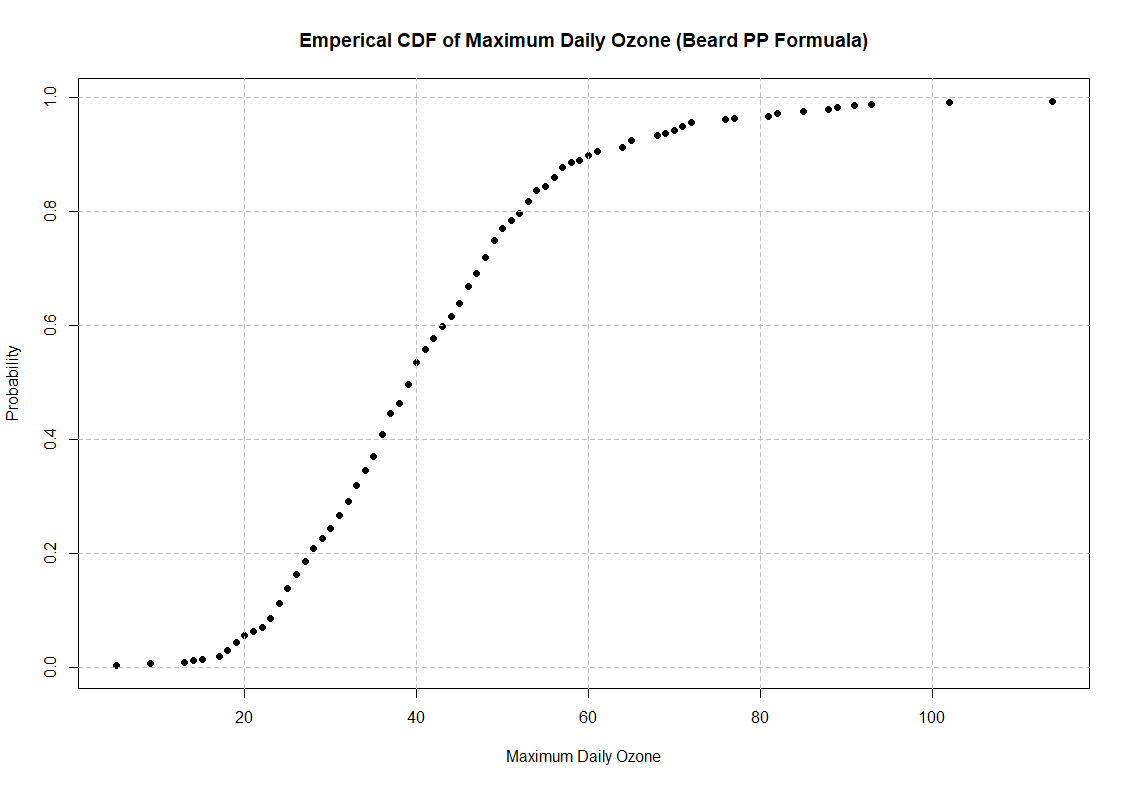
\includegraphics[width=0.95\textwidth]{Q1CDF}
	\caption{\footnotesize Empirical CDF for Maximum Daily Ozone using Beard Plotting Position Formula}
	\end{center}
\end{figure}

\pagebreak

\section *{Problem 2}
The objective is to plot the histogram of mean daily temperature using Freedman-Diaconis Binning Formula. The daily mean temperature value is average value aggregated from hourly data of each day.

\begin{figure} [H]
	\begin{center}
	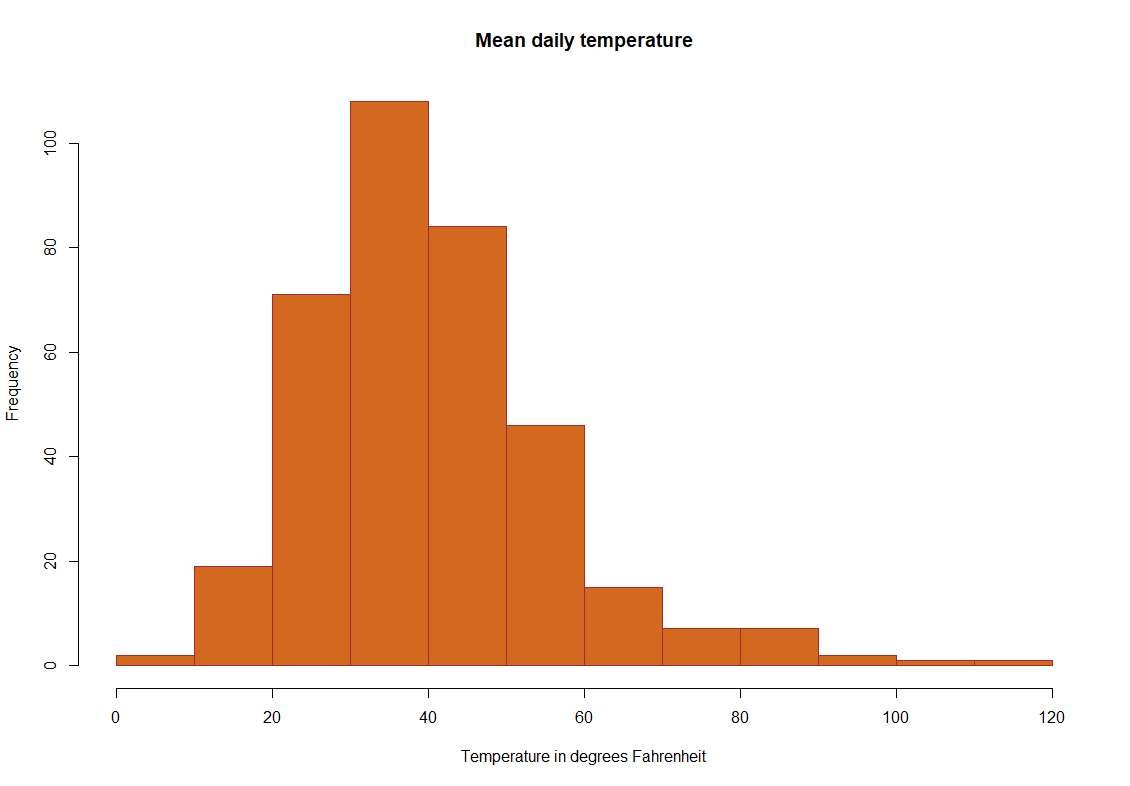
\includegraphics[width=0.95\textwidth]{Q2}
	\caption{\footnotesize Mean Daily Temperature's Histogram using Freedman-Diaconis Binning}
	\end{center}
\end{figure}


\section *{Problem 3}
The objective is to compute the 1\textsuperscript{st} ,5\textsuperscript{th}, 10\textsuperscript{th}, 25\textsuperscript{th}, 50\textsuperscript{th}, 75\textsuperscript{th}, 90\textsuperscript{th}, 95\textsuperscript{th}, 99\textsuperscript{th} percentile of daily maximum values of the oxides of nitrogen. The daily maximum value is aggregated into daily format from hourly data of oxides of nitrogen.

\begin{table}[H]
	\begin{center}
		\begin{tabular}{lllllllll}
\hline
\multicolumn{1}{|l|}{1\%}  & \multicolumn{1}{l|}{5\%}  & \multicolumn{1}{l|}{10\%} & \multicolumn{1}{l|}{25\%}  & \multicolumn{1}{l|}{50\%}  & \multicolumn{1}{l|}{75\%}  & \multicolumn{1}{l|}{90\%}  & \multicolumn{1}{l|}{95\%}  & \multicolumn{1}{l|}{99\%}   \\ \hline
\multicolumn{1}{|l|}{3.90} & \multicolumn{1}{l|}{7.70} & \multicolumn{1}{l|}{9.90} & \multicolumn{1}{l|}{15.20} & \multicolumn{1}{l|}{22.25} & \multicolumn{1}{l|}{36.50} & \multicolumn{1}{l|}{62.10} & \multicolumn{1}{l|}{87.60} & \multicolumn{1}{l|}{151.50} \\ \hline
		\end{tabular}
	\caption{\footnotesize Percentile Table for Daily Maximum Values of the Oxides of Nitrogen}	
	\end{center}
\end{table}

\pagebreak

\section *{Problem 4}
The objective is to create a correlation plot between Daily max Ozone, Daily min Dew Point Temperature,Maximum daily solar radiation, Maximum daily wind speed and Daily maximum concentration of oxides of nitrogen.

\begin{figure} [H]
	\begin{center}
	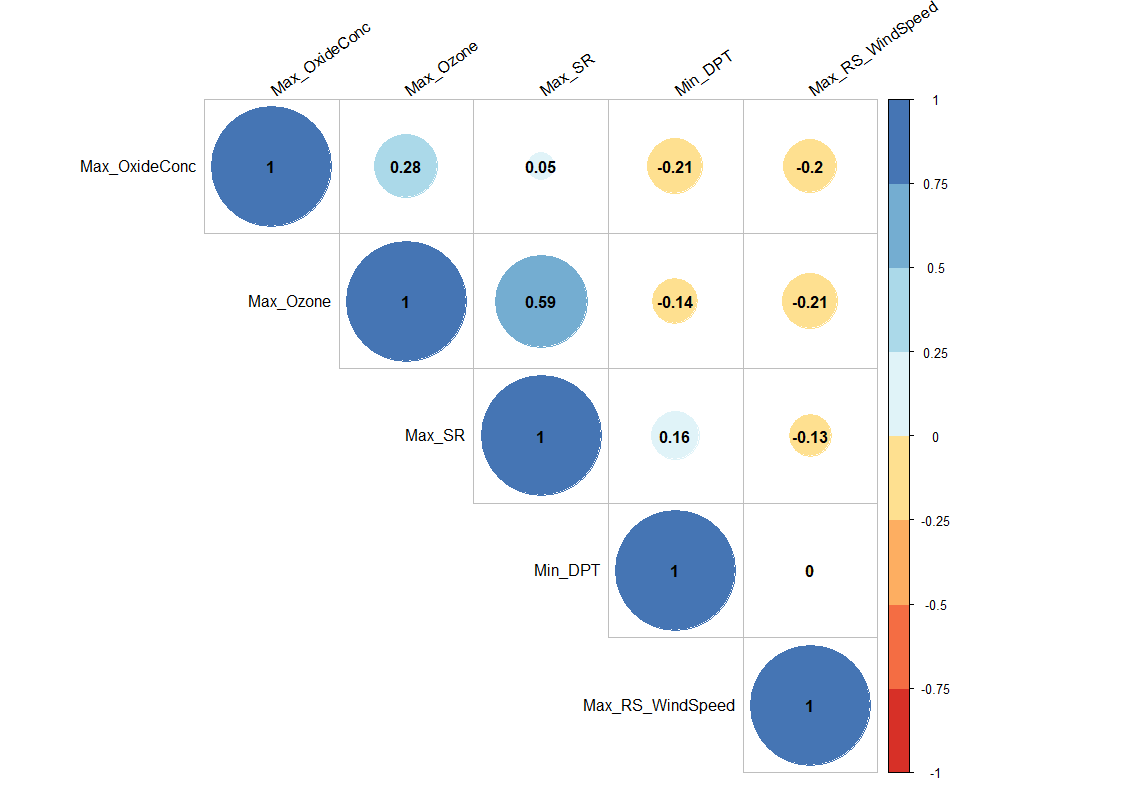
\includegraphics[width=1.1\textwidth]{Q3}
	\caption{\footnotesize Correlation plot using Spearman Rank Correlation Coefficient}
	\end{center}
\end{figure}

\begin{flushleft}
\textbf{Figure label Description} \linebreak
Max\textunderscore OxideConc - Daily Maximum Concentration of Oxides of Nitrogen \\
Max\textunderscore Ozone - Daily maximum Ozone Concentration \\
Max\textunderscore SR - Maximum Daily Solar Radiation \\
Min\textunderscore DPT - Daily Minimum Dew Point Temperature\\
Max\textunderscore RS\textunderscore WindSpeed - Maximum Daily Resultant Wind Speed\\ \pagebreak
\end{flushleft}

\section *{Problem 5}
The objective is to use 90 degree Quadrants of Wind Direction and compute the probability of Ozone being less than or
equal to 10 ppm or higher by creating a contingency table showing joint, marginal probabilities. Second, we will also compute the conditional probability for Ozone concentration being greater than 10ppb AND Resultant Wind Direction with 0 to 90 degrees. \\ \par 
\begin{center}
P(Ozone\textgreater 10 $|$ Wind Direction = NE(0 - 90]). \\ \par
\end{center}
Here, Ozone (POC 3) is measured in parts per billion and Resultant Wind Direction (POC 1) is measured in degrees compass with North as 0 degrees and South as 180 degrees. \\  \par

First, the count of all combined occurrences of Ozone level and Wind Direction Quadrant is arranged in the following table.

\begin{table}[H]
\begin{center}
\begin{tabular}{|c|c|c|c|c|}
\hline
\textbf{Ozone / WD}         & \textbf{NE} & \textbf{SE} & \textbf{SW} & \textbf{NW} \\ \hline
\textbf{\textless 10}       & 303         & 539         & 342         & 383         \\ \hline
\textbf{\textgreater{}= 10} & 1611        & 3191        & 942         & 1084        \\ \hline
\end{tabular}
\caption{\footnotesize Count of all combined occurrences of Ozone level and Wind Direction.}	
\end{center}
\end{table}

Contingency table showing all the joint and marginal probabilities is listed on following table.

\begin{table}[H]
	\begin{center}
		\begin{tabular}{|cl|cl|cl|cl|}
\hline
\multicolumn{2}{|c|}{\textbf{Ozone / WD}} & \multicolumn{2}{c|}{\textbf{\textless 10 ppb}} & \multicolumn{2}{c|}{\textbf{\textgreater = 10ppb}} & \multicolumn{2}{c|}{\textbf{Total}}      \\ \hline
\multicolumn{2}{|c|}{\textbf{0-90 Quad}}              & \multicolumn{2}{c|}{0.03609291}            & \multicolumn{2}{c|}{0.19189994}                      & \multicolumn{2}{c|}{\textbf{0.22799285}} \\ \hline
\multicolumn{2}{|c|}{\textbf{90-180 Quad}}            & \multicolumn{2}{c|}{0.06420488}            & \multicolumn{2}{c|}{0.38010721}                      & \multicolumn{2}{c|}{\textbf{0.44431209}} \\ \hline
\multicolumn{2}{|c|}{\textbf{180-270 Quad}}           & \multicolumn{2}{c|}{{0.04073853}}   & \multicolumn{2}{c|}{{0.11220965}}             & \multicolumn{2}{c|}{\textbf{0.15294818}} \\ \hline
\multicolumn{2}{|c|}{\textbf{270-360 Quad}}           & \multicolumn{2}{c|}{0.04562239}            & \multicolumn{2}{c|}{0.12912448}                      & \multicolumn{2}{c|}{\textbf{0.17474687}} \\ \hline
\multicolumn{2}{|c|}{\textbf{Total}}                  & \multicolumn{2}{c|}{0.1866587}             & \multicolumn{2}{c|}{0.8133413}                       & \multicolumn{2}{c|}{\textbf{1}}          \\ \hline
		\end{tabular}
	\caption{\footnotesize Contingency table showing all joint and marginal probabilities.}	
	\end{center}
\end{table}

\end{document}